\documentclass[journal, onecolumn, final, letterpaper, 11pt]{IEEEtran}
\usepackage{setspace}

\usepackage{cite}
\usepackage{amsmath}
\usepackage{mathtools}
\usepackage{svg}
\usepackage{epstopdf}
\usepackage{float}
\usepackage{wrapfig}
\usepackage[center]{caption}

\font\myfont=cmr12 at 18pt

\begin{spacing}{1.0}
\title{\myfont{\textmd{A Full State Feedback Controller for Dynamic Capacitive Wireless Power Transfer Systems}}}
\normalsize
\end{spacing}

\begin{document}
\maketitle
 
\doublespacing

\vspace{-0.85cm}
\begin{spacing}{1.4}
\noindent \textbf{{\small Abstract}} -- \small{This digest presents a novel full-state feedback (FSF) controller for compensating changing coupling variations in dynamic capacitive wireless power transfer (WPT) systems utilizing an active variable reactance (AVR) rectifier. The AVR rectifier enables continuous compensation, allowing the WPT system to maintain high-efficiency power transfer at a fixed frequency by appropriately distributing power between its two branches. Conventional PID control is suboptimal for the AVR rectifier due to the higher-order system dynamics, nonlinearities, and cross-coupling between control loops. In contrast, the FSF control strategy presents an optimal and robust way to control higher order multi-input multi-output systems like the AVR rectifier. A state-space model is developed for the AVR rectifier, and the FSF controller is designed based on this model. To validate the proposed approach, a 13.56 MHz 100-W capacitive WPT system with an AVR rectifier is built and tested. The controller’s effectiveness is demonstrated through both simulations and experiments on the hardware prototype.}
\end{spacing}

\vspace{-0.15cm}

\section{Introduction}

Wireless power transfer (WPT) is becoming increasingly important and has the potential to accelerate the widespread adoption of electric vehicles (EVs), especially amongst vehicles that routinely travel along fixed routes such as buses and warehouse forklifts. Capacitive WPT systems can be lighter, cheaper, and smaller than comparable inductive WPT systems due to the absence of ferrite cores. The ability of capacitive WPT systems to transfer high power at high efficiency has been demonstrated, thus proving the viability of this technology \cite{2023_Maji_WPTCE}.

One main challenge of WPT systems is the extreme sensitivity to the value of the coupling capacitance or mutual inductance between the receiver and the transmitter. To increase the practicality of WPT systems in dynamic applications, it is desirable to design and control them to tolerate coupling variations while maintaining full power transfer at high efficiency. The recently proposed active variable reactance (AVR) rectifier addresses these challenges and efficiently provides variable compensation in high-frequency WPT systems \cite{2019_Sinha_Journal}. However, a robust controller is needed in order to perform this compensation automatically and with a sufficiently high bandwidth to allow for in-motion dynamic EV charging. A conventional PID control-based decoupled-dual-loop strategy has been proposed to compensate for changing coupling capacitance while maintaining the desired power transfer \cite{2019_Sinha_ECCE, 2024_Maji_COMPEL}. However, such approaches are not well-suited to optimally control the AVR rectifier due to the higher-order system dynamics, nonlinearities, and cross-coupling between the two control loops.

This work presents a novel time-domain solution for the control of the AVR rectifier with sufficiently high bandwidth and robustness to operate the system dynamically. First, a model of the AVR rectifier is derived in state space. Then, a state-space control strategy is proposed, and an optimal full state feedback (FSF) linear quadratic regulator (LQR) controller is designed and validated in simulation. Finally, a prototype 13.56-MHz, 100-W capacitive WPT system with an AVR rectifier and a dynamically variable coupling capacitance is built and its operation demonstrated with the proposed control strategy.

\begin{figure*}[!ht]
	\vspace{-0.7cm}
	\centering
	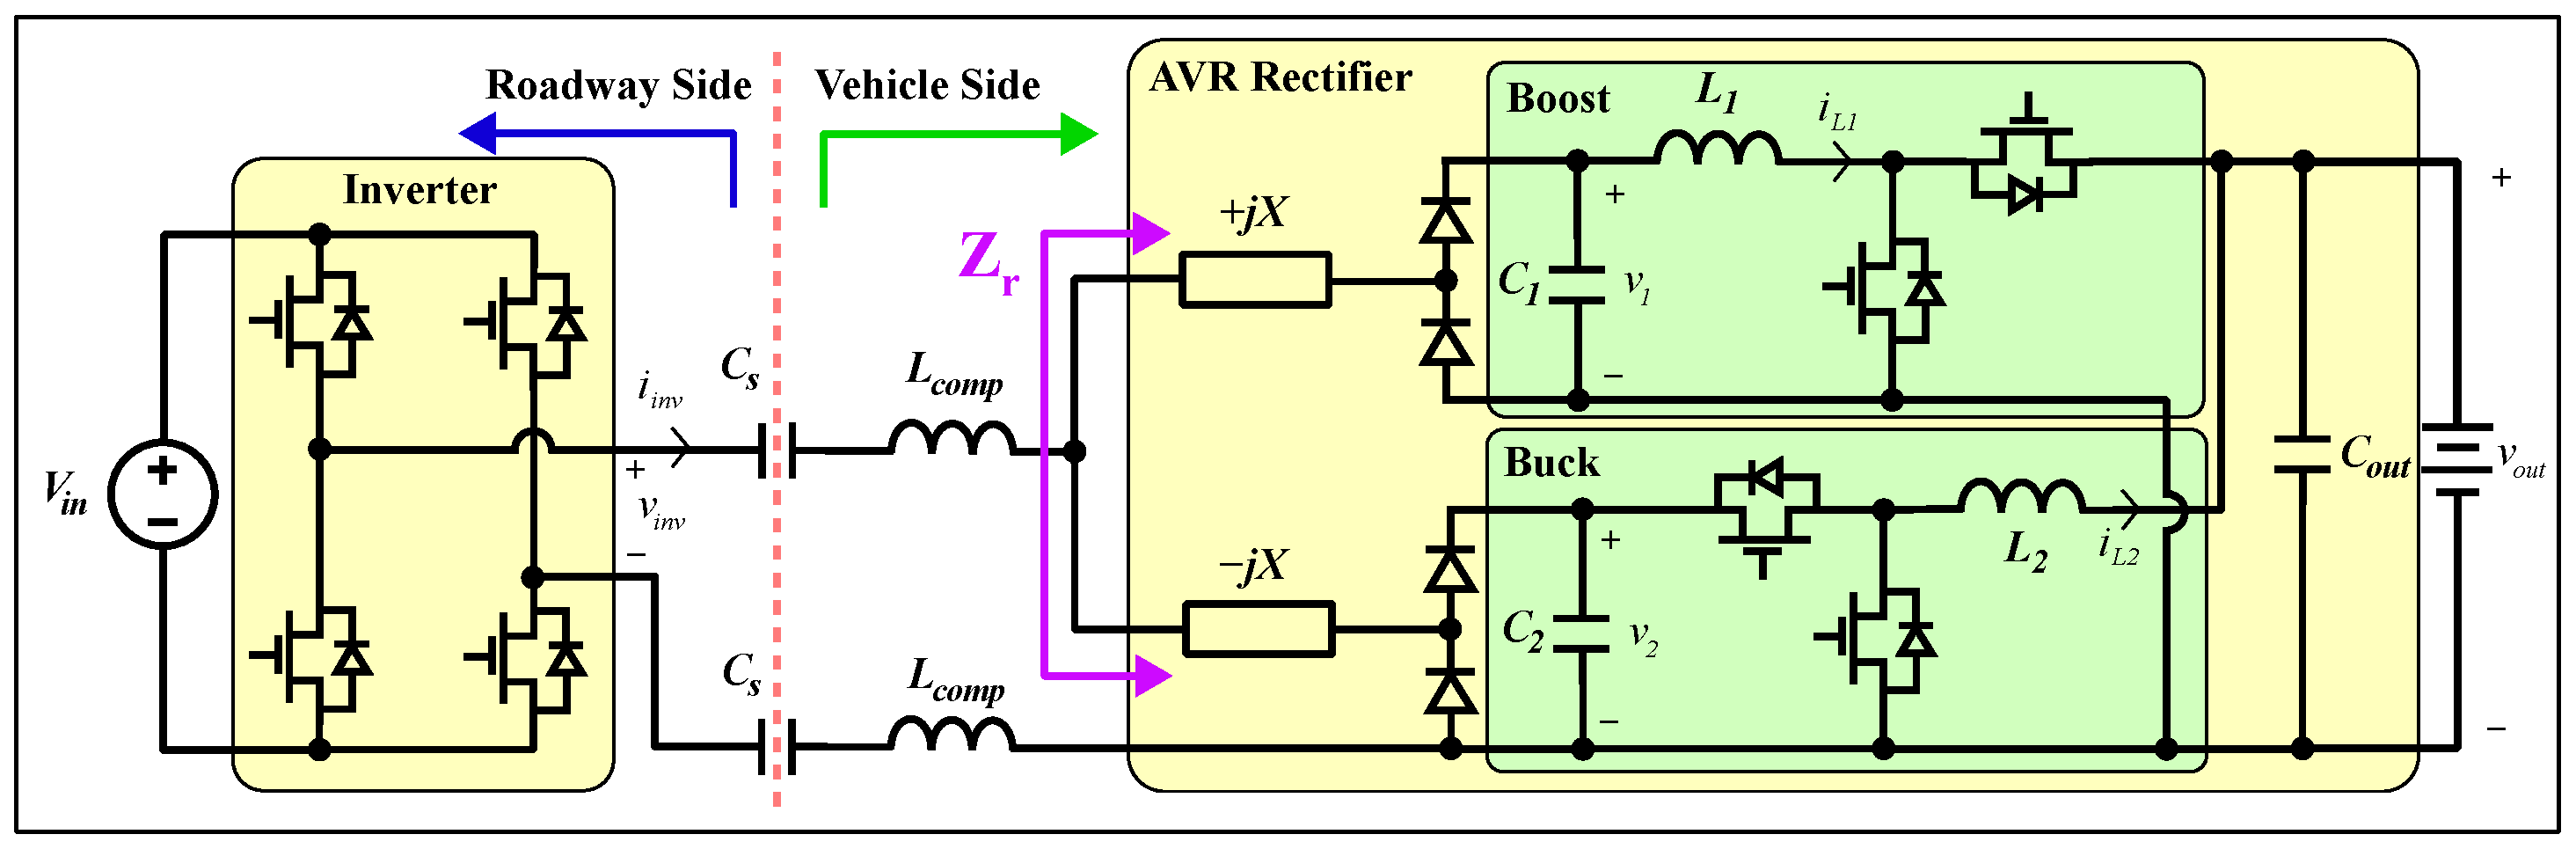
\includegraphics[width=0.85\textwidth]{figures/wpt_with_avr_full_schematic_eps.eps}
	\caption{Dynamic capacitive wireless power transfer system with active variable reactance rectifier schematic.}
	\label{fig:full_schematic}
	
	\vspace{-0.5cm}
\end{figure*}

\section{Dynamic Capacitive Wireless Power Transfer System with an AVR Rectifier}
\label{sec:system}

Figure \ref{fig:full_schematic} presents the circuit schematic of the dynamic capacitive WPT system with the AVR rectifier. A DC input bus is connected to a full-bridge inverter. Power then flows through the $L_{comp}C_s$ tank. $C_s$ is the coupling capacitance between the roadway-side and vehicle-side coupling plates; $L_{comp}$ is designed such that the impedance of the series-resonant LC tank is zero when $C_s$ assumes its nominal value $C_{s,nom}$.

The AVR rectifier has two branches: a top branch containing a boost converter attached to an inductive reactance $+jX$, and a bottom branch containing a buck converter attached to a capacitive reactance $-jX$. By independently varying the amount of power processed in each branch, the AVR rectifier can maintain the desired constant output power ($P_{out})$ while compensating for coupling variations by modulating the impedance seen at the input of the AVR rectifier ($z_r$). Throughout this digest, the following notation is used: $p_{out}$ is the time-varying measured variable, $P_{out}$ is the constant nominal DC value, and $\widehat{p_{out}}$ is the small-signal variable. They are related as $p_{out}(t) \equiv P_{out} + \widehat{p_{out}}(t)$. Equations \ref{eqn:pout}-\ref{eqn:zin} give $p_{out}$ and $z_r$ as a function of the large-signal circuit states as labeled in Fig. \ref{fig:full_schematic}:

\footnotesize
\vspace{-0.8cm}
\begin{subequations}\label{eqn:pout_zin}
	\begin{align}
		p_{out} &= p_1 + p_2 = v_1 i_{L1} + v_{out} i_{L2} \label{eqn:pout} \\
		z_r &= \operatorname{Re}(z_r) + j\cdot\operatorname{Im}(z_r) = r_r + jx_r = \frac{k_{rec}^2 v_1^2 v_2^2 + v_1v_{out}i_{L1}i_{L2}X^2}{k_{rec}(v_1v_2^2i_{L1} + v_{out}v_1^2i_{L2})} + jX\frac{v_1 i_{L1}v_2^2 - v_{out} i_{L2}v_1^2}{v_1 i_{L1}v_2^2 + v_{out} i_{L2}v_1^2} \label{eqn:zin}
	\end{align}
\end{subequations}
\normalsize

\vspace{-0.2cm}

$k_{rec}$ is a gain associated with the half-bridge rectifiers under sinusoidal approximation, and $X$ is the differential reactance $\pm jX$ attached to the two branches. When the coupling capacitance $C_s$ changes by an amount $\Delta C_s$, Eqn. \ref{eqn:zin} is utilized to adjust the operation of the AVR rectifier such that $x_r$ perfectly compensates $\Delta C_s$ while maintaining $r_r = R_r$. This also guarantees $p_{out} = P_{out}$, as well as resistive loading on the inverter.

A frequency-based controller has been proposed in \cite{2024_Maji_COMPEL} which utilizes two control loops: one maintains $p_{out} = P_{out}$, and the other maintains $r_r = R_r$. The two loops run at the same frequency, but use constant decoupling gains to minimize cross-coupling between the loops. However, the controller does not have sufficient performance to operate the system in dynamic charging scenarios. FSF controllers are typically more robust than conventional PID controllers and thus suitable for the class of control problems that the AVR rectifier falls into: relativey nonlinear, heavily-coupled multi-input multi-output (MIMO) systems. The FSF controller designed in this work follows the same control strategy of attempting to hold $p_{out}$ and $r_r$ constant at their nominal values $P_{out}$ and $R_r$.

\section{State Space Modeling of the AVR Rectifier}
\label{sec:modeling}

In this section, a model for the AVR rectifier is developed in state space using a method similar to that employed in \cite{2010_Mayo_CONIELECOMP}. Sec. \ref{sec:control} uses this model for the design of a robust FSF controller. Figure \ref{fig:small_signal} contains the small-signal linearized model of the AVR rectifier. Of note is the inclusion of the input capacitance on both of the converters; these capacitors are necessary in modeling the dynamics of the converter as the input voltages $v_1$ and $v_2$ vary.

In general, a continuous-time state-space model can be written as $\frac{d}{dt}\vec{x} = A\vec{x} + B\vec{u}$, where $\vec{x}$ is the state vector, $\vec{u}$ is the input vector, $A$ is the system dynamics matrix, and $B$ is the input dynamics matrix. The AVR rectifier state-space model is derived from its small-signal model, so the state vector $\widehat{\vec{x}}$ contains the small-signal voltages and currents $\widehat{v_1}, \widehat{v_2}, \widehat{i_{L1}}, \widehat{i_{L2}}$, and $\widehat{v_{out}}$, as labeled in Fig. \ref{fig:small_signal}. The input vector $\widehat{\vec{u}}$ contains the small-signal control handles $\widehat{d_1}$ and $\widehat{d_2}$, which correspond to the small-signal duty cycles of the boost and the buck converters, respectively.

First-order differential equations for $\frac{d}{dt}\widehat{\vec{x}}$ are written using time-domain circuit analysis techniques. These are arranged into a matrix, resulting in a valid five-state un-augmented state space model of the AVR rectifier. However, the controller design requires additional augmented integral states $z_1 \equiv \int_0^t \widehat{p_{out}}(\tau) d\tau$ and $z_2 \equiv \int_0^t \widehat{r_r}(\tau) d\tau$ which track the integral of the error in output power $p_{out}(t)$ and error in the real part of the input impedance $r_r(t)$, respectively. $\widehat{p_{out}}$ and $\widehat{r_r}$ can be computed from the elements of $\widehat{\vec{x}}$ using Eqns. \ref{eqn:pout}-\ref{eqn:zin}. Thus, an augmented state vector $\overrightarrow{x_{aug}} = \begin{bsmallmatrix} \vec{x} & z_1 & z_2 \end{bsmallmatrix}^T$ can be constructed, and the complete state-space model becomes Eqn. \ref{eqn:aug_ss_model}. This model is the first significant contribution of this digest, and a derivation will be presented in the full paper.

\vspace{-0.1cm}

\scriptsize
\begin{equation}
\label{eqn:aug_ss_model}
\frac{d}{dt}
\begin{bmatrix}
	\widehat{v_{out}} \\
	\widehat{v_1} \\
	\widehat{v_2} \\
	\widehat{i_{L1}} \\
	\widehat{i_{L2}} \\
	z_1 \\
	z_2
\end{bmatrix}
=
\begin{bmatrix}
	-\frac{1}{RC_{out}} & 0 & 0 & \frac{D_1'}{C_{out}} & \frac{1}{C_{out}} & 0 & 0 \\
	0 & 0 & 0 & -\frac{1}{C_1} & 0 & 0 & 0 \\
	0 & 0 & 0 & 0 & -\frac{D_2}{C_2} & 0 & 0\\
	-\frac{D_1'}{L_1} & \frac{1}{L_1} & 0 & 0 & 0 & 0 & 0 \\
	-\frac{1}{L_2} & 0 & \frac{D_2}{L_2} & 0 & 0 & 0 & 0 \\
	-I_{L2} & -I_{L1} & 0 & -V_1 & -V_{out} & 0 & 0 \\
	-\frac{\partial r_r}{\partial v_{out}} & -\frac{\partial r_r}{\partial v_{1}} & -\frac{\partial r_r}{\partial v_{2}} & -\frac{\partial r_r}{\partial i_{L1}} & -\frac{\partial r_r}{\partial i_{L2}} & 0 & 0
\end{bmatrix}
\begin{bmatrix}
	\widehat{v_{out}} \\
	\widehat{v_1} \\
	\widehat{v_2} \\
	\widehat{i_{L1}} \\
	\widehat{i_{L2}} \\
	z_1 \\
	z_2
\end{bmatrix}
+
\begin{bmatrix}
	-\frac{I_{L1}}{C_{out}} & 0 \\
	0 & 0 \\
	0 & -\frac{I_{L2}}{C_2} \\
	\frac{V_{out}}{L_1} & 0 \\
	0 & \frac{V_2}{L_2} \\
	0 & 0 \\
	0 & 0
\end{bmatrix}
\begin{bmatrix}
	\widehat{d_1} \\
	\widehat{d_2}
\end{bmatrix}
\end{equation}
\normalsize

\begin{figure}[b]
\vspace{-0.4 cm}
\centering
\begin{minipage}{.5\textwidth}
  \centering
  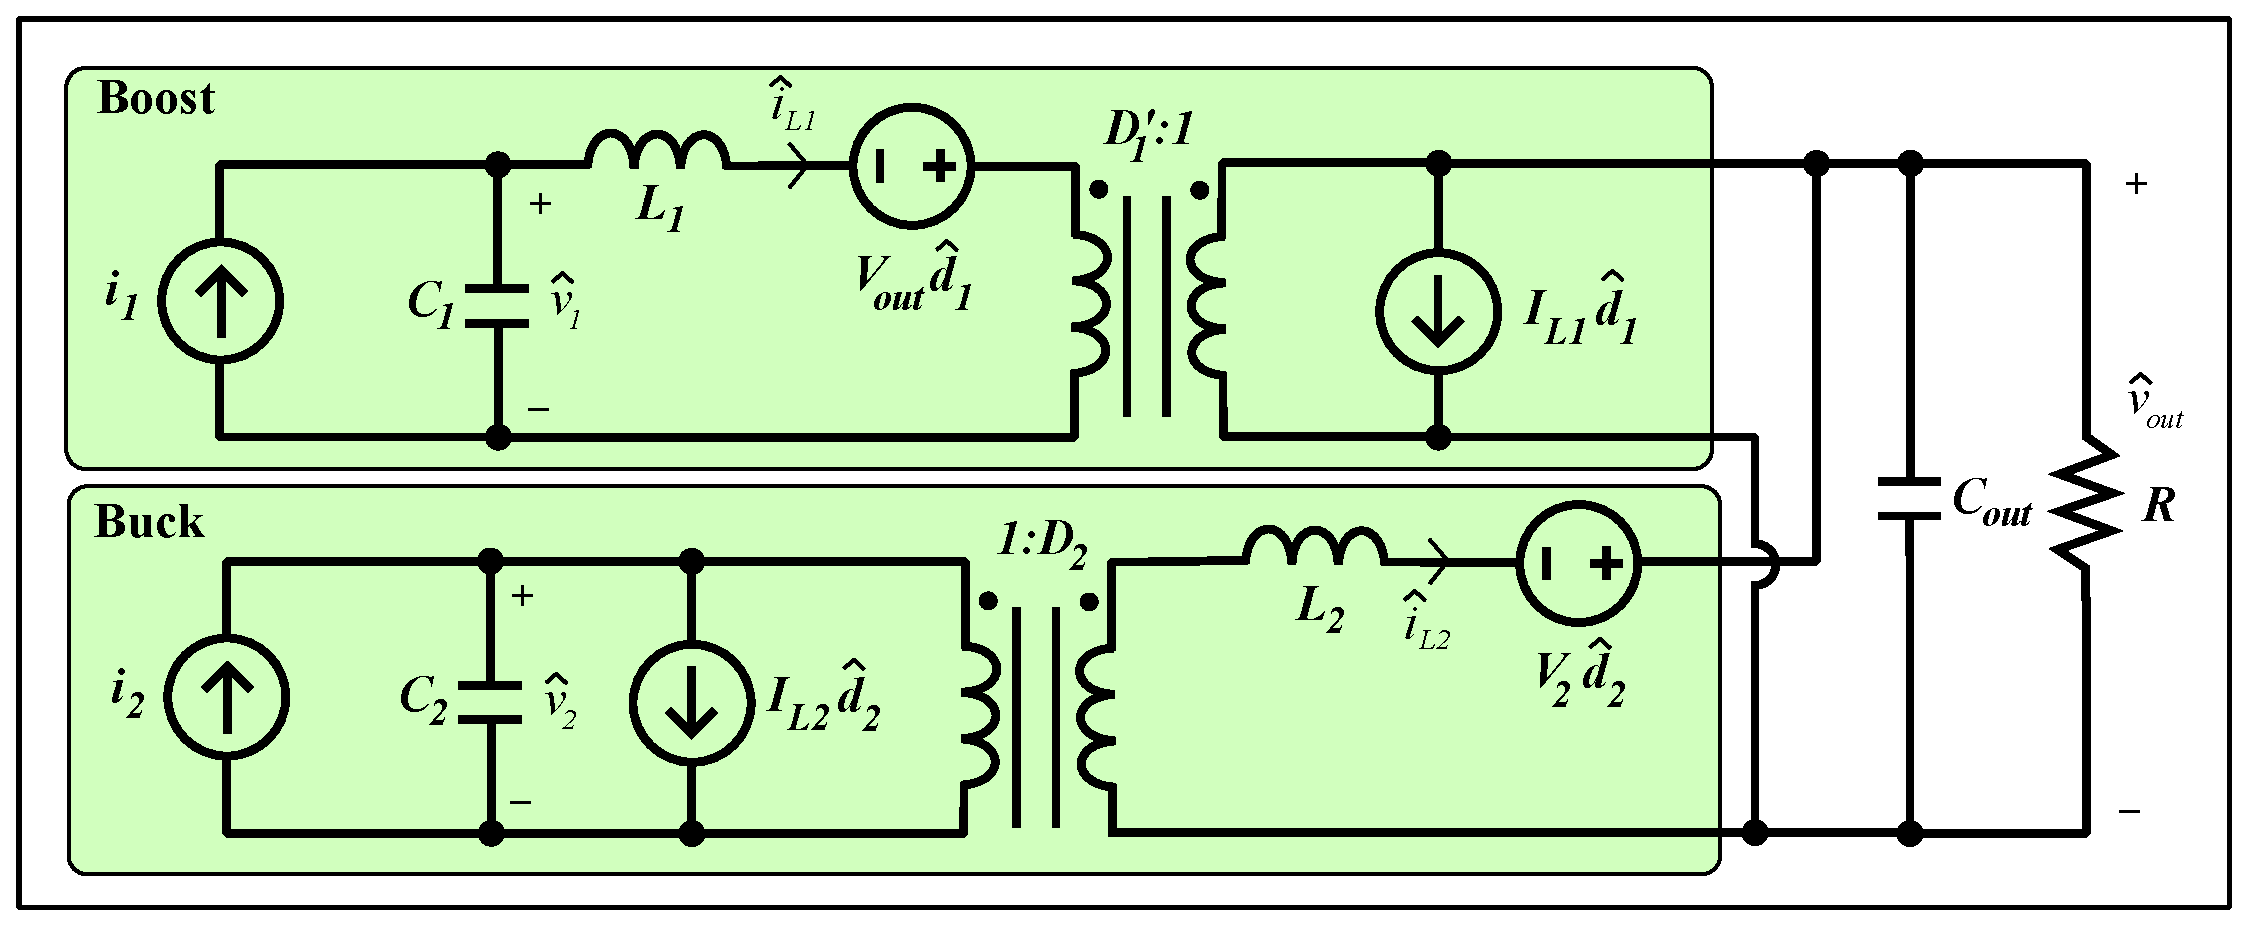
\includegraphics[width=\linewidth]{figures/avr_ss_model_schematic_eps.eps}
  \caption{Schematic of the AVR rectifier's linearized small-signal model.}
  \label{fig:small_signal}
\end{minipage}%
\begin{minipage}{.5\textwidth}
  \centering
  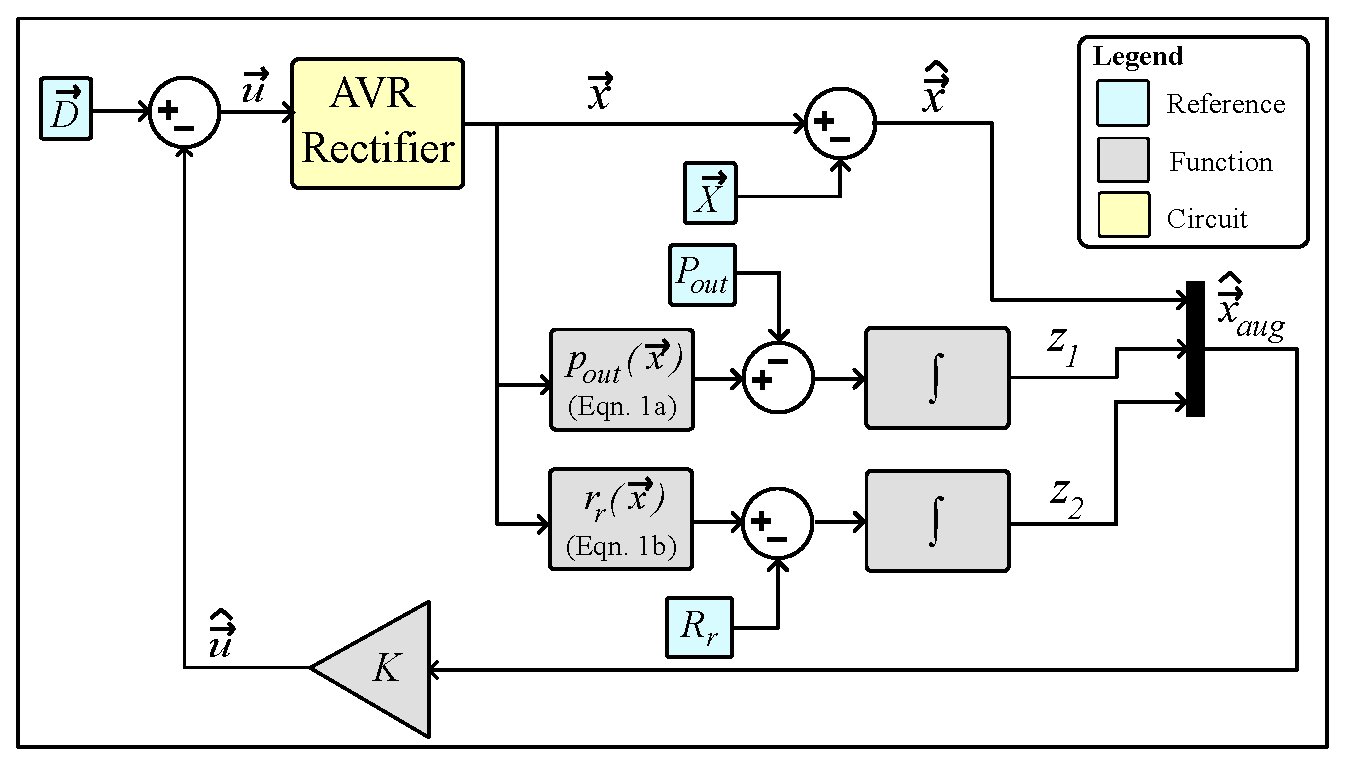
\includegraphics[width=0.95\linewidth]{figures/block_diagram_eps.eps}
  \caption{Simplified block diagram of the state-space control loop. $p_{out}(\vec{x})$ is given by Eqn. \ref{eqn:pout}; $r_r(\vec{x})$ is given by Eqn. \ref{eqn:zin}, $\vec{D}$ is the vector of nominal duty ratios for the buck and boost converters.}
  \label{fig:block_diagram}
\end{minipage}
\vspace{-0.4cm}
\end{figure}

\section{Full State Feedback Controller Design and Simulation Validation}
\label{sec:control}

Figure \ref{fig:block_diagram} shows the complete block diagram of the system under closed-loop control. The controller design consists of finding a gain matrix $K$ such that setting the input as $\vec{u} = \vec{D} - K\overrightarrow{x_{aug}}$ results in the closed-loop system driving $p_{out}$ and $r_r$ to their nominal values $P_{out}$ and $R_r$ regardless of the value of $C_s$. To find an optimal $K$, heuristic techniques presented in \cite{2007_Williams} are used to design a linear quadratic regulator (LQR) with reasonable values for the diagonal elements of the $Q$ and $R$ cost-defining matrices. Then, the \texttt{lqr()} function in MATLAB is utilized to solve the corresponding Algebraic Riccati Equation for the optimal gain matrix $K$. The strategy for choosing $Q$ and $R$ will be presented in the full paper.

\begin{figure*}[!b]
	\vspace{-0.2cm}
	\centering
	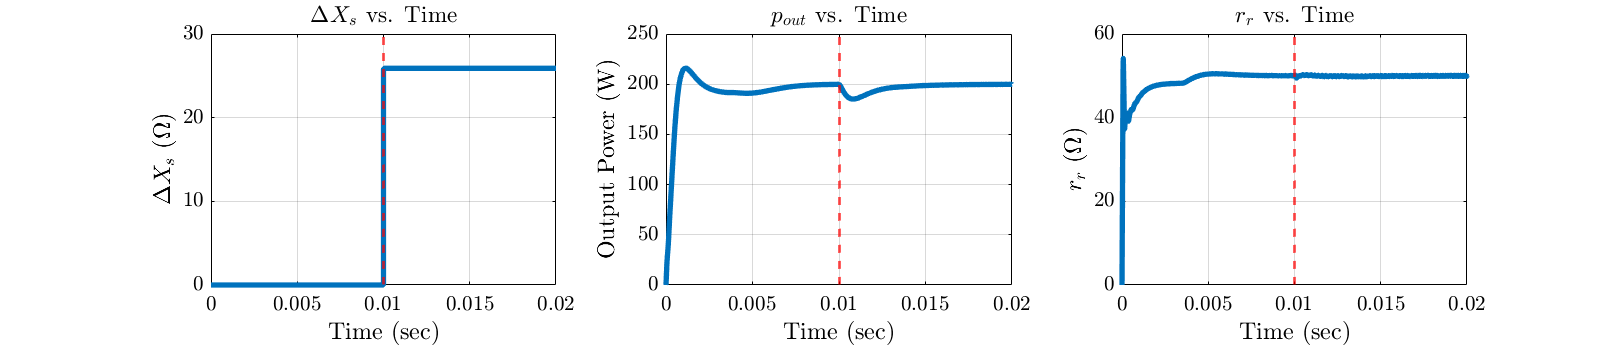
\includegraphics[width=\textwidth]{figures/pout_zin_with_disturbance.png}
	\caption{$p_{out}$ and $r_r$ vs. time, showing the AVR rectifier's startup transient under the proposed controller for $t \in [0, 0.01)$, followed by a step change in coupling reactance $\Delta X_s$ at time $t = 0.01$.}
	\label{fig:step_response}
\end{figure*}

A model is built in Simulink and PLECS to validate the proposed controller. Figure \ref{fig:step_response} shows the control objectives $p_{out}$ and $r_r$ being controlled to their target values of $P_{out} = 200 \texttt{ }W$ and $R_r = 50 \texttt{ }\Omega$, respectively, while the coupling reactance is disturbed by an amount $\Delta X_s \equiv \frac{1}{2 \pi f_s}(\frac{1}{C_{s,nom}} - \frac{1}{C_s})$, where $f_s$ is the switching frequency, and $C_{s,nom}$ is the nominal coupling capacitance. The impedance seen by the inverter must be near-resistive for the converter to operate at peak efficiency. Figure \ref{fig:input_waveforms} shows the inverter output voltage ($v_{inv}$) and inverter output current ($i_{inv}$) waveforms under a misalignment condition with and without the controller. The proposed controller is enabling the AVR rectifier to compensate for a change in coupling reactance, as shown by the inverter output voltage and current waveforms being nearly in-phase. The design of the FSF controller for the AVR rectifier and simulation results showing its effectiveness are the second significant contribution of this work.

\begin{figure*}[!b]
	\centering
	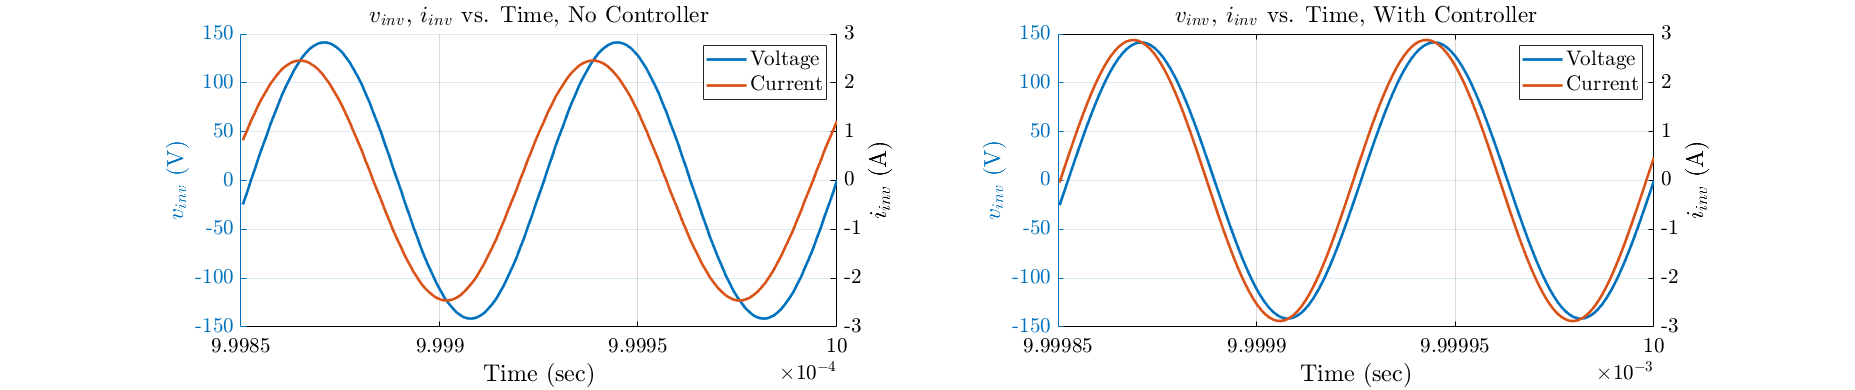
\includegraphics[width=\textwidth]{figures/input_waveforms_with_without_control.png}
	\caption{Inverter output voltage $v_{inv}$ and inverter output current $i_{inv}$ with a change in coupling reactance $\Delta X_s = 26 \Omega$, with and without the controller.}
	\label{fig:input_waveforms}
\end{figure*}

\section{Hardware and Experimental Results}
\label{sec:hardware}

\begin{figure}[t]
\centering
\begin{minipage}{.55\textwidth}
  \centering
  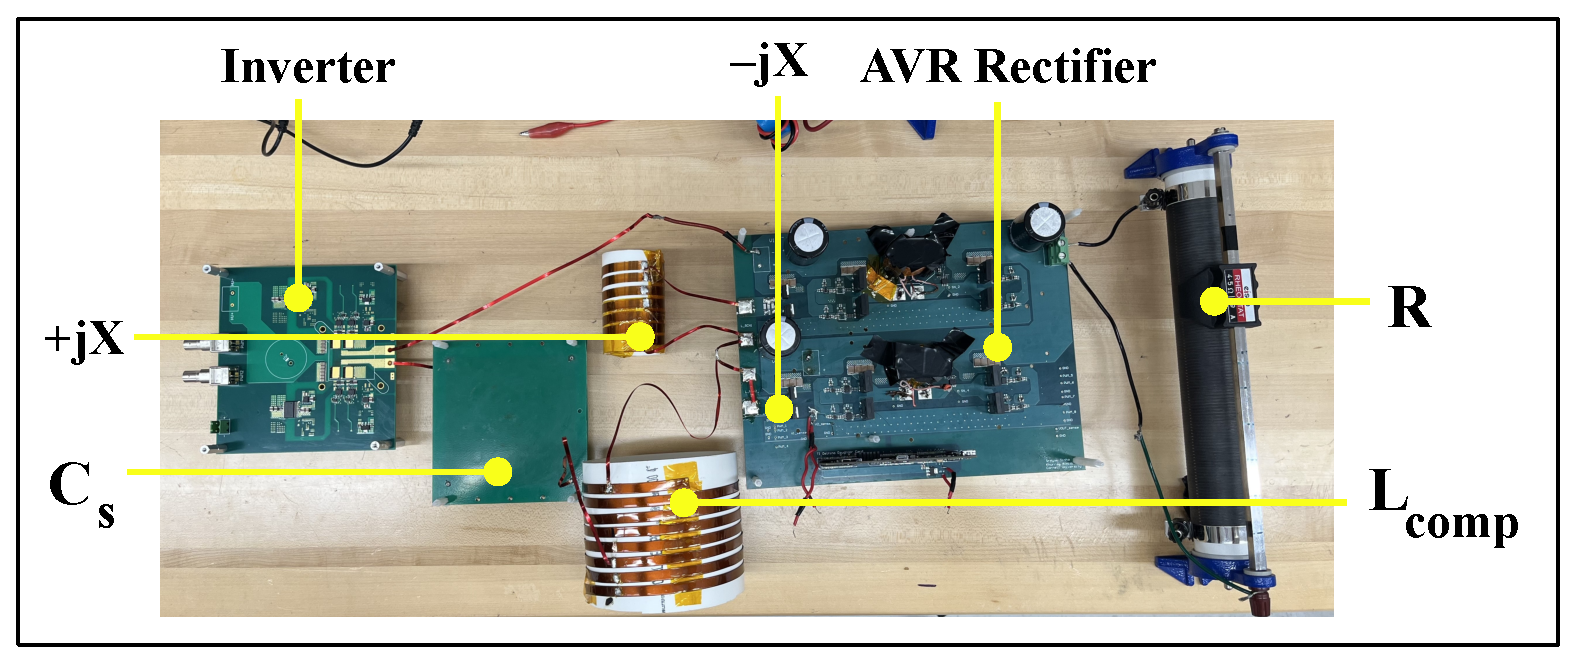
\includegraphics[width=0.95\textwidth]{figures/prototype_annotated_eps.eps}
	\caption{Annotated photograph of the hardware prototype. A load resistor $R$ is used in place of a battery.}
  \label{fig:hardware_prototype}
\end{minipage}%
\begin{minipage}{0.45\textwidth}
  \centering
  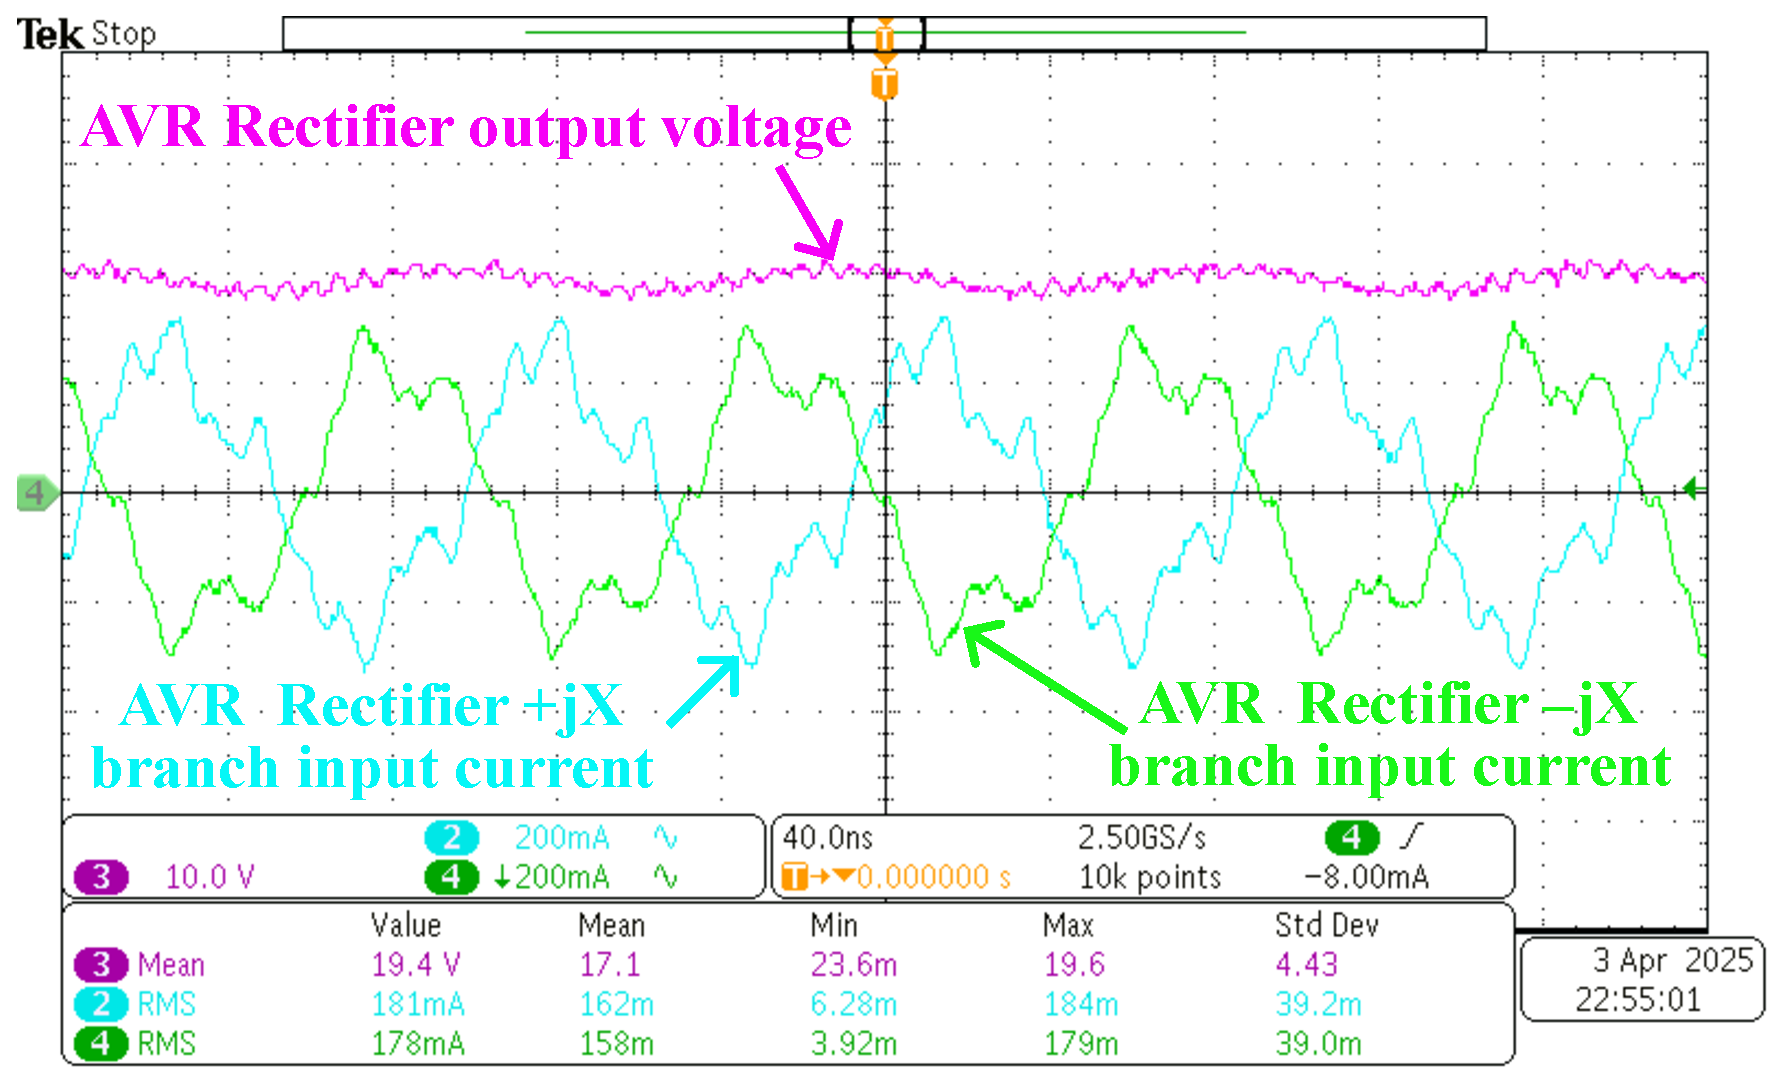
\includegraphics[width=0.95\textwidth]{figures/avr_waveforms_annotated_eps.eps}
	\caption{Experimental waveforms showing AVR rectifier branch currents and output voltage.}
  \label{fig:waveform}
\end{minipage}
\vspace{-0.4cm}
\end{figure}

The proposed controller is implemented on a prototype 13.56 MHz, 100-W capacitive WPT system equipped with an AVR rectifier and a dynamically adjustable coupling capacitance. Figure \ref{fig:hardware_prototype} shows the hardware prototype and experimental setup with annotations labeling important components. An exhaustive list of components used will be provided in the full paper. Figure \ref{fig:waveform} shows AVR rectifier waveforms with $\Delta C_s = 0$ and $V_{in} = 30 \text{ } V$. The current flowing into the AVR rectifier is being split evenly between the $+jX$ and $-jX$ branches, showing nominal operation. Experimental waveforms with the controller enabled will be provided in the full paper. The controller implementation and experimental results showing controller effectiveness comprise the third significant contribution of this work.

\section{Conclusion and Future Work}
\label{sec:conclusion}

This digest presents a novel state-space model and full state feedback (FSF) controller for capacitive WPT systems equipped with AVR rectifiers. The proposed controller allows the system to transfer power efficiently as the coupling capacitance between the transmitter and receiver is varied. A 13.56-MHz, 100-W capacitive WPT system with an AVR rectifier and a dynamically adjustable coupling capacitance was assembled. The proposed controller was validated in simulation and on the hardware prototype.

\footnotesize
\begin{spacing}{1.0}
\bibliographystyle{ieeetr}
\bibliography{refs}
\end{spacing}

\end{document}